\documentclass{article}
\usepackage[a4paper, left=3cm, right=2cm, top=3cm, bottom=2cm]{geometry}
\usepackage{graphicx}
\usepackage{amsmath}
\usepackage[shortlabels]{enumitem}
\usepackage{array}
\usepackage{xcolor}
\usepackage{amssymb}
\usepackage{amsthm}
\usepackage{mathtools}
\usepackage{tikz}
\usepackage{pgfplots}
\usepackage{arydshln}


\pgfplotsset{compat=1.18} % Set pgfplots compatibility level



\title{
    \textbf{Universidade de São Paulo\\ Escola Politécnica}\\
    \vspace{20pt}
    
\includegraphics[scale=0.5]{images/logo-poli.png} \\
    \vspace{20pt}
    \textbf{PNV5761 - Programação Matemática Aplicada a Problemas de Transporte} \\
    \vspace{10pt}
    \textbf{Segunda série de problemas.}\\
    \vspace{15pt}
    \large{Prof. Marco Antonio Brinati} \\
    \vspace{45pt}
    % \large{Guilherme Fernandes Alves - 10774361} \\
    \vspace{10pt}
    \date{\textbf{\Large{São Paulo, Agosto de 2024}}}
}

\author{Guilherme Fernandes Alves - 10774361}

\begin{document}

\renewcommand{\arraystretch}{1.5}

\maketitle
\newpage

\section{Questão 1}

Escreva a forma canônica do problema de programação linear descrito abaixo em termos das variáveis básicas (dependentes) $x_{1}$, $x_{2}$ e $x_{3}$ e o represente no plano das variáveis não básicas (independentes) $x_{4}$ e $x_{5}$, identificando a solução ótima.
Compare o resultado com aquele visto em aula, para o qual as variáveis básicas eram $x_{3}$, $x_{4}$ e $x_{5}$.

\[
  \begin{array}{r@{}r@{}r@{}r@{}r@{}r}
    \text{Min} \quad z =           -4x_1 &{} +            6x_2 &{} + 6x_3 &{} - 4x_4 &{} + \frac{9}{2}x_5 \\[\jot]
    \text{s.t.}\quad\quad           4x_1 &{} +  \frac{5}{6}x_2 &{} + 3x_3 &{} + 2x_4 &{} +           4x_5 &{} = 29\\
                                   -2x_1 &{} + \frac{23}{6}x_2 &{} + 3x_3 &{} - 2x_4 &{} +           4x_5 &{} = 11\\
                         -\frac{7}{2}x_1 &{} +            7x_2 &{} + 6x_3 &{} - 4x_4 &{} +           6x_5 &{} = 18\\

    \multicolumn{4}{c}{x_j \geq 0, \quad j=1,..., 5}
  \end{array}
\]

\subsection{Solução}

Primeiramente, destacamos que o problema já está na forma padrão.

Começamos a resolver através do método de eliminação de Gauss-Jordan, de modo que as variáveis básicas sejam $x_{1}$, $x_{2}$ e $x_{3}$.
Sendo assim, começamos a escrever a matriz aumentada do sistema de equações:

\[
\renewcommand{\arraystretch}{1.5}
\begin{array}{|ccccc:c|}
             x_1 &          x_2 &         x_3 &         x_4 & x_5 & b \\ \hline
               4 &  \frac{5}{6} &           3 &           2 &   4 & 29 \\
    -          2 & \frac{23}{6} &           3 &          -2 &   4 & 11 \\
    -\frac{7}{2} & 7            &           6 &          -4 &   6 & 18 \\ \hdashline
              -4 & 6            &           6 &          -4 &  \frac{9}{2} &  
  \end{array}
\]

Normalização da primeira linha: Dividir a primeira linha por 4 para transformar o coeficiente de $x_1$ em 1:

\[
\renewcommand{\arraystretch}{1.5}
\begin{array}{|ccccc:c|}
             x_1 &          x_2 &         x_3 &         x_4 & x_5 & b \\ \hline
               1 & \frac{5}{24} & \frac{3}{4} & \frac{1}{2} &   1 & \frac{29}{4} \\
    -          2 & \frac{23}{6} &           3 &          -2 &   4 & 11 \\
    -\frac{7}{2} & 7            &           6 &          -4 &   6 & 18 \\ \hdashline
              -4 & 6            &           6 &          -4 &  \frac{9}{2} &  
  \end{array}
\]

Normalização de x1 nas linhas 2 e 3: Adicionar 2 vezes a primeira linha à segunda linha e $\frac{7}{2}$ vezes a primeira linha à terceira linha para zerar os coeficientes de $x_1$ nas demais linhas.

\[
\renewcommand{\arraystretch}{1.5}
\begin{array}{|ccccc:c|}
  x_1 &          x_2 &         x_3 &         x_4 & x_5 & b \\ \hline
    1 & \frac{5}{24} & \frac{3}{4} & \frac{1}{2} & 1 & \frac{29}{4}\\
    0 & \frac{17}{4} & \frac{9}{2} & -1 & 6 & \frac{51}{2}\\
    0 & \frac{371}{48} & \frac{69}{8} & -\frac{9}{4} & \frac{19}{2} & \frac{347}{8} \\ \hdashline
   -4 & 6            &           6 &          -4 &  \frac{9}{2} &  
  \end{array}
\]

Normalização de $x_2$: Multiplicar linha 2 por $\frac{4}{17}$ para obter 1 na variável $x_2$.
Multiplicar linha 2 por $\frac{5}{24}$ e subtrair da linha 1 para zerar o coeficiente de $x_2$ na linha 1.
Multiplicar linha 2 por $\frac{371}{48}$ e subtrair da linha 3 para zerar o coeficiente de $x_2$ na linha 3.

\[
\renewcommand{\arraystretch}{1.5}
\begin{array}{|ccccc:c|}
  x_1 & x_2 &           x_3 &            x_4 &             x_5 &  b \\ \hline
    1 &   0 &  \frac{9}{17} &  \frac{28}{51} &   \frac{12}{17} &  6 \\
    0 &   1 & \frac{18}{17} &  -\frac{4}{17} &   \frac{24}{17} &  6 \\
    0 &   0 & \frac{15}{34} & -\frac{22}{51} &  -\frac{24}{17} & -3 \\ \hdashline
   -4 &   0 &             6 &             -4 &     \frac{9}{2} &  
  \end{array}
\]

Normalização da coluna de $x_3$:
Multiplicar linha 3 por $\frac{34}{15}$ para obter 1 na variável $x_3$.
Multiplicar linha 3 por $\frac{9}{17}$ e subtraindo da linha 1 para zerar o coeficiente de $x_3$ na linha 1.
Multiplicar linha 3 por $\frac{18}{17}$ e subtraindo da linha 2 para zerar o coeficiente de $x_3$ na linha 2.

\[
\renewcommand{\arraystretch}{1.5}
\begin{array}{|ccccc:c|}
  x_1 & x_2 & x_3 & x_4 & x_5 & b \\ \hline
    1 & 0 & 0 &  \frac{16}{15} &  \frac{12}{15} &  \frac{48}{5} \\
    0 & 1 & 0 &    \frac{4}{5} &   \frac{24}{5} &  \frac{66}{5} \\
    0 & 0 & 1 & -\frac{44}{45} &  -\frac{16}{5} & -\frac{34}{5} \\ \hdashline
   -4 & 0 & 6 &             -4 &    \frac{9}{2} &
  \end{array}
\]

Dessa forma, já podemos visualizar o modelo na forma canônica.
E a partir dele podemos gerar a representação geométrica do problema, dado que nenhuma das variáveis básicas é negativa.

\begin{figure}[h]
  \centering
  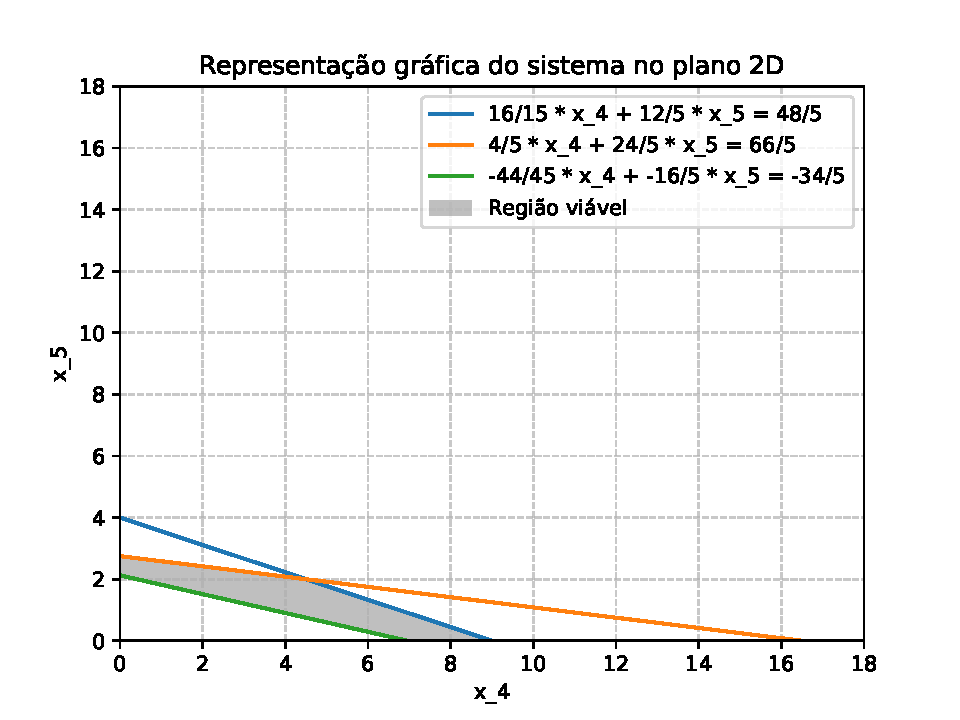
\includegraphics[width=0.6\textwidth]{images/Q1-grafico.pdf}
  \caption{Representação geométrica do problema 1}
\end{figure}

Podemos escrever a função objetivo em termos das variáveis básicas:

\begin{align}
  z &= -4x_1 + 6x_2 + 6x_3 - 4x_4 + \frac{9}{2}x_5 \notag\\
  &= -4 \cdot \left( \frac{48}{5} - \frac{16}{15} x_4 - \frac{12}{15} x_5 \right) \notag\\
  &\quad + 6 \cdot \left( \frac{66}{5} - \frac{4}{5} x_4 - \frac{24}{5} x_5 \right) \notag\\
  &\quad + 6 \cdot \left( -\frac{34}{5} + \frac{44}{45} x_4 + \frac{16}{5} x_5 \right) \notag\\
  &\quad - 4x_4 + \frac{9}{2}x_5 \\
  &= \frac{4}{3} \cdot x_4 - \frac{19}{10} \cdot x_5 \notag
\end{align}

Sendo assim, podemos utilizar a expressão acima para determinar visualmente a solução ótima do problema.
Vejamos:

\begin{figure}[h]
  \centering
  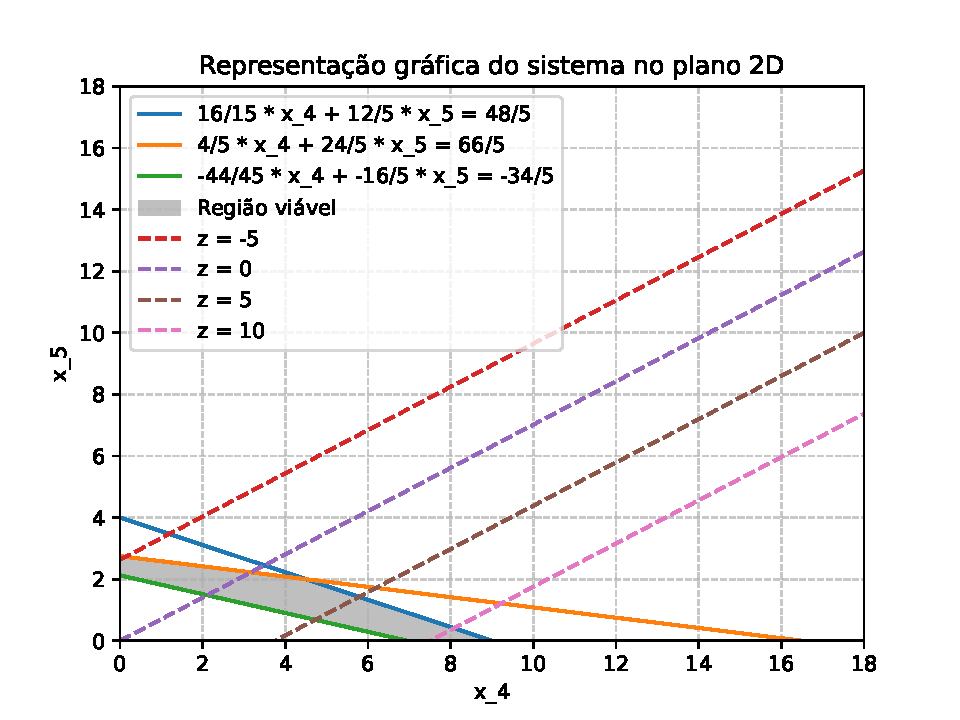
\includegraphics[width=0.6\textwidth]{images/Q1-grafico-com-z.pdf}
  \caption{Representação geométrica do problema 1}
\end{figure}

Pela figura acima, podemos ver que a solução ótima corresponde ao vértice em que a reta laranja cruza o eixo vertical ($x_4 = 0$), ou seja, quando $x_4 = 0$ e $x_5 = \frac{11}{4}$, visto que o objetivo é minimizar a função $z$.
Deste modo, a solução ótima será $z = \frac{4}{3} \cdot 0 - \frac{19}{10} \cdot \frac{11}{4} = \frac{-209}{40} = - 5.225$

Quando comparamos com a solução apresentada em aula, vemos que a solução ótima é a mesma, porém desta vez a função objetivo e a forma geométrica da região viável foram apresentadas de forma diferente.
Aqui notamos que a escolha de variáveis básicas pode influenciar na forma como o problema é visualizado e, eventualmente, alterar o número de iterações necessárias para encontrar a solução ótima.
Se não tivermos um método estruturado para escolher as variáveis básicas, podemos acabar tendo que realizar mais iterações do método simplex para encontrar a solução ótima.

\section{Questão 2}

Seja $x^{\prime}$ uma solução viável para o problema de programação linear na forma padrão cuja função objetivo é limitada inferiormente na região viável.
Admita que:

\begin{enumerate}
  \item $x^{\prime}_{1} > 0, \quad x^{\prime}_{2} > 0, \dots, x_{r}^{\prime} > 0, x_{r+1}^{\prime} > 0, x_{r+2}^{\prime} = x_{r+3}^{\prime}=\cdots, x_{n}^{\prime}=0$ 
  \item $A_{r+1} = \alpha_{1} \cdot A_{1} + \alpha_{2} \cdot A_{2} + \dots + \alpha_{r} \cdot A_{r}$ (isto é, a coluna $A_{r+1}$ da variável $x^{\prime}_{r+1}$ no sistema de equações $Ax = b$ é uma combinação linear das colunas $A_{1}, A_{2}, \dots, A_{r}$)
\end{enumerate}

Mostre, então, que existe uma solução viável $y$ cujo número de componentes positivas é menor ou igual a $r$, tal que $c \cdot y \leq c \cdot x_{\prime}$.
Sugestão: Faça $y = x_{\prime} + \theta \cdot v$, com $v = \left[ \alpha_{1}, \alpha_{2}, \dots, \alpha_{r}, -1, 0, 0, 0, \dots, 0 \right]^{T}$.

Comentário: A partir do resultado deste exercício, é fácil mostrar que, para procurar uma solução ótima para o PPL na forma padrão, basta examinar as soluções viáveis, $x$, cujas componentes positivas $x_j$ estejam associadas a colunas $A_j$ da matriz $A_j$ linearmente independentes (que é a maneira que utilizamos para obter uma solução básica).

\section{Questão 3}

Considere para o problema de programação linear da Questão 1 a solução viável   
$x_{1}^{\prime} = 2, x_{2}^{\prime} = 6, x_{3}^{\prime} = \frac{2}{3}, x_{4}^{\prime}$ e $x_{5}^{\prime}$.
Considere agora a proposta da Questão 2 de obter uma solução $y$ melhor que $x^{\prime}$ para a Questão 1.
Como há infinitas soluções para o sistema de equações:

\[
  A_5 = \alpha_1 \cdot A_1 + \alpha_2 \cdot A_2 + \alpha_3 \cdot A_3 + \alpha_4 \cdot A_4
\]

Arbitre $\alpha_4$ e calcule os valores de $\alpha_1, \alpha_2, \alpha_3$.
Determine a seguir,

\begin{enumerate}[(a)]
    \item O sinal de $\theta$ para $cy< cx^{\prime}$, e depois
    \item O valor de $\theta$ para que o número de componentes positivos de $y$ seja menor que o de $x^{\prime}$.
\end{enumerate}

\section{Questão 4}

Programação Linear 

\begin{enumerate}[(a)]
  \item Admita-se conhecido um modelo de programação linear associado a um problema de nutrição. Neste problema de nutrição, deseja-se minimizar o custo de uma dieta diária, partindo-se de uma cesta de 12 alimentos diferentes para atender os requisitos mínimos de 5 nutrientes diferentes. Você espera que a solução ótima venha contemplar o consumo de todos esses alimentos? Justifique.
  \item Quando uma variável $x_j$ é irrestrita em sinal, faz-se a substituição de $x_j$ por duas outras variáveis $x_{j}^{+}$ e $x_{j}^{-}$ tais que: $x_j = x_{j}^{+} - x_{j}^{-}; \quad x_{j}^{+} \geq 0 ; \quad x_{j}^{-} \geq 0$
\end{enumerate}
 
Mostre que o simplex não examina nenhuma solução em que $x_{j}^{+}$ e $x_{j}^{-}$ sejam simultaneamente positivas.

\subsection{Solução}

\subsubsection{Item (a)}

Trata-se de um problema de 12 variáveis de decisão e 5 restrições.
Neste caso, a matriz $A$ terá dimensões $5 \times 12 = 60$ e, portanto, terá no máximo 5 linhas linearmente independentes (L.I.).
Deste modo, a matriz $A$ não será inversível, o que implica que a solução ótima não contemplará o consumo de todos os alimentos.

% Conforme vimos em aula, a solução ótima será uma solução básica degenerada, ou seja, uma solução em que a matriz $A$ não é inversível.

% \subsubsection{Item (b)}

\section{Questão 5}

\begin{enumerate}[(a)]
    \item Num problema de programação linear, somente os vértices (as soluções básicas) podem ser solução ótima?
    \item Se o conjunto de soluções viáveis de um problema de programação linear for um conjunto não limitado, o problema pode ter uma solução ótima?
    \item Um problema de programação linear na forma padrão, com $m$ restrições e $n$ variáveis possui sempre $\binom{n}{m}$ soluções básicas viáveis?
    \item Dada uma solução básica degenerada, qual é a condição para que a próxima tabela do simplex corresponda a um novo vértice?
\end{enumerate}

\subsection{Solução}

\begin{enumerate}[(a)]
    \item Sim, somente os vértices (ou soluções básicas) podem ser soluções ótimas em um problema de programação linear. Isto é verdade porque, no método simplex, as soluções são movidas de um vértice para outro ao longo das arestas do politopo de soluções viáveis. Como a função objetivo é linear, se ela atinge um valor ótimo, esse valor deve ocorrer em um vértice ou em uma aresta que liga dois vértices ótimos. Se houver múltiplas soluções ótimas, elas estarão localizadas em uma aresta ou face do politopo, mas os vértices adjacentes a essa aresta ou face ainda serão soluções ótimas.
    \item Sim, um problema de programação linear pode ter uma solução ótima mesmo que o conjunto de soluções viáveis não seja limitado, mas isso depende da direção da função objetivo. Se a função objetivo for otimizada (minimizada ou maximizada) em uma direção onde o conjunto de soluções viáveis não é limitado, o problema não terá uma solução ótima finita (o valor da função objetivo pode ser infinitamente grande ou pequeno). No entanto, se a direção da otimização for contrária à região não limitada, o problema pode ter uma solução ótima finita.
    \item Não, um problema de programação linear não possui necessariamente $\binom{n}{m}$ soluções básicas viáveis. O número $\binom{n}{m}$ representa o número de soluções básicas possíveis, mas nem todas essas soluções básicas são necessariamente viáveis (isto é, satisfazem as restrições de não negatividade e as equações do sistema). Algumas dessas soluções básicas podem ter componentes negativas ou podem ser não viáveis por outras razões, resultando em menos soluções básicas viáveis do que $\binom{n}{m}$.
    \item Quando uma solução básica é degenerada (ou seja, uma ou mais variáveis básicas são iguais a zero), a próxima tabela do simplex pode corresponder ao mesmo vértice (solução básica) se não houver uma melhora na função objetivo. Isso ocorre quando a movimentação ao longo de uma direção básica não altera o valor da função objetivo, resultando em um ciclo ou na permanência no mesmo vértice. Para que a próxima tabela corresponda a um novo vértice, é necessário que haja uma mudança na base que resulte em um deslocamento para um vértice diferente. Na prática, isso significa que uma variável básica com valor zero deve sair da base, e uma nova variável deve entrar, alterando o conjunto de variáveis básicas.
\end{enumerate}

\section{Questão 6}

% - pra ser nao básica, precisa ter 2 vertices

\begin{enumerate}[(a)]
    \item Como a existência de uma solução não básica ótima pode ser identificada da tabela do simplex?
    \item Quando se reconhece numa tabela do simplex que a função objetivo é ilimitada inferiormente na região viável?
    \item Numa iteração do simplex, a variável $x_2$ foi retirada da base: $x_2$ poderá voltar à base na iteração seguinte?
\end{enumerate}

\subsection{Solução}

\begin{enumerate}[(a)]
  \item Uma solução não básica ótima pode ser identificada na tabela do simplex quando todos os coeficientes na linha da função objetivo (linha \( z \)) são não negativos (ou seja, \( c_j - z_j \geq 0 \) para todas as variáveis não básicas). Neste caso, a solução atual é ótima. Se houver coeficientes nulos (\( c_j - z_j = 0 \)) correspondentes a variáveis não básicas, isso indica que existe uma solução ótima alternativa onde essas variáveis não básicas poderiam entrar na base sem alterar o valor da função objetivo. Essa situação é característica de múltiplas soluções ótimas, e a solução ótima alternativa seria uma solução não básica.
  \item A função objetivo é reconhecida como ilimitada inferiormente na região viável em uma tabela do simplex quando, ao escolher uma coluna pivô (ou seja, uma coluna com um coeficiente negativo na linha \( z \) que poderia melhorar a função objetivo), todas as razões \( \frac{b_i}{a_{ij}} \) (onde \( a_{ij} > 0 \)) são negativas ou indefinidas (ou seja, \( a_{ij} \leq 0 \) para todos os \( i \)). Isso significa que, ao aumentar a variável correspondente à coluna pivô, a solução pode crescer indefinidamente sem violar nenhuma restrição, o que implica que a função objetivo pode ser minimizada sem limite, ou seja, é ilimitada inferiormente.
  \item Sim, a variável \( x_2 \) pode voltar à base na iteração seguinte, dependendo das condições da tabela. Se, na próxima iteração, a variável \( x_2 \) se tornar a candidata que proporciona a maior melhora na função objetivo (ou a menor degradação, no caso de maximização) e for escolhida como a variável entrante, ela poderá reentrar na base. Isso é comum em problemas onde há degenerescência, ou seja, onde múltiplas soluções básicas correspondem ao mesmo valor da função objetivo. Nessas situações, uma variável pode sair e voltar à base em iterações subsequentes.
\end{enumerate}

\section{Questão 7}
% - Depende da solução dual

Resolver, utilizando o algoritmo simplex e, se necessário, o método das duas fases, os seguintes problemas de programação linear.

\subsection{Problema a}

\[
  \begin{array}{r@{}r@{}r@{}r@{}r@{}r}
    \text{Max} \quad z =   2x_1 &{} + 2x_2 &{} + 4x_3 &{} \\[\jot]
    \text{s.t.}\quad\quad  5x_1 &{} + 2x_2 &{} - 1x_3 &{} \leq 6\\
                           2x_1 &{} + 8x_2 &{} + 2x_3 &{} \leq 6\\
                          -2x_1 &{} + 4x_2 &{} + 2x_3 &{} \leq 4\\

    \multicolumn{4}{c}{x_j \geq 0, \quad j=1, 2, 3}
  \end{array}
\]

\subsubsection{Solução}

Primeiramente, queremos transformar o problema em um problema de minimização, multiplicando a função objetivo por $-1$.

\[
  \begin{array}{r@{}r@{}r@{}r@{}r@{}r}
    \text{Min} \quad z =  -2x_1 &{} - 2x_2 &{} - 4x_3 &{} \\[\jot]
    \text{s.t.}\quad\quad  5x_1 &{} + 2x_2 &{} - 1x_3 &{} \leq 6\\
                           2x_1 &{} + 8x_2 &{} + 2x_3 &{} \leq 6\\
                          -2x_1 &{} + 4x_2 &{} + 2x_3 &{} \leq 4\\

    \multicolumn{4}{c}{x_j \geq 0, \quad j=1, 2, 3}
  \end{array}
\]

Agora, como as restrições são do tipo desigualdade, precisamos adicionar variáveis de folga para transformar em um problema de igualdade.

\[
  \begin{array}{r@{}r@{}r@{}r@{}r@{}r@{}r}
    \text{Min} \quad z =  -2x_1 &{} - 2x_2 &{} - 4x_3 &{} \\[\jot]
    \text{s.t.}\quad\quad  5x_1 &{} + 2x_2 &{} - 1x_3 &{} + s_1 &{} = 6\\
                           2x_1 &{} + 8x_2 &{} + 2x_3 &{} + s_2 &{} = 6\\
                          -2x_1 &{} + 4x_2 &{} + 2x_3 &{} + s_3 &{} = 4\\

    \multicolumn{5}{c}{x_j, s_j \geq 0, \quad j=1, 2, 3}
  \end{array}
\]

Agora que o problema está na forma padrão, montamos a tabela inicial do simplex, onde cada linha representa uma restrição, e a última linha (linha \(z\)) representa a função objetivo.

\[
  \begin{array}{c|cccccc|c}
    \text{base} & x_1 & x_2 & x_3 & s_1 & s_2 & s_3 & b  \\ \hline
            s_1 &   5 &   2 &  -1 &   1 &   0 &   0 &        6 \\
            s_2 &   2 &   8 &   2 &   0 &   1 &   0 &        6 \\
            s_3 &  -2 &   4 &   \color{red}2\color{black} &   0 &   0 &   1 &        4 \\ \hline
              z &  -2 &  -2 &  -4 &   0 &   0 &   0 &        0
  \end{array}
\]

Agora, analisamos a tabela para identificar a variável que entra na base e a que sai. A variável \(x_3\) é escolhida para entrar na base porque ela tem o coeficiente mais negativo na linha \(z\), o que indica que aumentá-la mais pode melhorar o valor da função objetivo. A variável $s_3$ sai base, pois a razão \( \frac{b_i}{a_{ij}} \) é a menor positiva, assim determinando o pivô que está marcado em $Ameo$.

\[
  \begin{array}{c|cccccc|c}
    \text{base}                       & x_1 & x_2 & x_3 & s_1 & s_2 &         s_3 & b \\ \hline
    s_1 &                           4 &   4 &   0 &   1 &   0 & \frac{1}{2} & 8 \\
    s_2 &  \color{red}4 \color{black} &   4 &   0 &   0 &   1 &          -1 & 2 \\
    x_3 &                          -1 &   2 &   1 &   0 &   0 & \frac{1}{2} & 2 \\ \hline
      z &                          -6 &   6 &   0 &   0 &   0 &           2 & 8
  \end{array}
\]

Na segunda iteração, a variável $x_1$ é escolhida para entrar na base, pois ela tem o coeficiente negativo mais significativo na linha \(z\). A variável $s_2$ sai da base pois a razão \( \frac{b_i}{a_{ij}} \) é a menor positiva, determinando o pivô como sendo o elemento \(a_{22}\).


\[
  \begin{array}{c|cccccc|c}
    \text{base} & x_1 & x_2 & x_3 & s_1 & s_2 &         s_3 & b \\ \hline
    s_1 &   0 &   0 &   0 &   1 &   -1 & \frac{3}{2} & 6 \\
    x_1 &   1 &   1 &   0 &   0 &  \frac{1}{4} &  -\frac{1}{4} & \frac{1}{2} \\
    x_3 &   0 &   3 &   1 &   0 &   \frac{1}{4} & \frac{1}{4} & \frac{5}{2} \\ \hline
      z &   0 &  12 &   0 &   0 &   \frac{3}{2} & \frac{1}{2} & 11
  \end{array}
\]

A solução ótima é encontrada quando não há mais coeficientes negativos na linha z, indicando que o valor da função objetivo não pode ser mais reduzido. Neste caso, a solução ótima é 
$z = 11$ e $x_1 = \frac{1}{2}, x_2 = 0, x_3 = \frac{5}{2}, S_1 = 6, S_2 = 0, S_3 = 0$.


\subsection{Problema b}

\[
  \begin{array}{r@{}r@{}r@{}r@{}r@{}r}
    \text{Min} \quad z =  8x_1 &{} - 6x_2 &{} - 10x_3 &{} \\[\jot]
    \text{s.t.}\quad\quad 0x_1 &{} + 2x_2 &{} - 4x_3 &{} \leq 8\\
                          1x_1 &{} + 1x_2 &{} + 1x_3 &{} \geq 4\\
                          0x_1 &{} + 1x_2 &{} - 1x_3 &{} \geq -2\\

    \multicolumn{4}{c}{x_j \geq 0, \quad j=1, 2, 3}
  \end{array}
\]

\subsubsection{Solução}

Primeiramente precisamos adaptar o problema para a forma padrão, adicionando as variáveis de folga e/ou artificiais em cada uma das restrições.
Na restrição 1, que possui o sinal $\leq$, adicionamos a variável de folga $s_1$.
Na restrição 2, que possui o sinal $\geq$, adicionamos a variável de folga $s_2$ e adicionamos a variável artificial $A_1$.
Na restrição 3, o termo independente é negativo, então multiplicamos todos os coeficientes por $-1$ para inverter o sinal, e então adicionamos a variável de folga $s_3$.
Como o problema possui variáveis artificiais, utilizamos o método das duas fases para resolver.
Na primeira fase, a função objetivo busca minimizar a soma das variáveis artificiais.

Segue a formulação do problema na forma padrão:

\[
  \begin{array}{c|ccccccc|c}
    \text{base} &                       x_1 & x_2 & x_3 & s_1 & s_2 & s_3 & A_1 &  b \\ \hline
            s_1 &                         0 &   2 &  -4 &   1 &   0 &   0 &   0 &  8 \\
            A_1 & \color{red}1\color{black} &   1 &   1 &   0 &  -1 &   0 &   1 &  4 \\
            s_3 &                         0 &  -1 &   1 &   0 &   0 &   1 &   0 &  2 \\ \hline
              z &                        -1 &  -1 &  -1 &   0 &   1 &   0 &   0 & -4
  \end{array}
\]

Escolhemos a variável $x_1$ para entrar na base e a variável $A_1$ para sair da base.
O elemento pivô é 1, que está marcado em vermelho.

\[
  \begin{array}{c|ccccccc|c}
    \text{base} & x_1 & x_2 & x_3 & s_1 & s_2 & s_3 & A_1 &  b \\ \hline
            s_1 &   0 &   2 &  -4 &   1 &   0 &   0 &   0 &  8 \\
            x_1 &   1 &   1 &   1 &   0 &  -1 &   0 &   1 &  4 \\
            s_3 &   0 &  -1 &   1 &   0 &   0 &   1 &   0 &  2 \\ \hline
              z &   0 &   0 &   0 &   0 &   0 &   0 &  -1 &  0
  \end{array}
\]

As iterações da primeira fase terminam, pois não há mais variáveis artificiais na base.
Isso indica uma solução ótima para a primeira fase, mas precisamos verificar se a solução é viável para o problema original.
Eliminamos as variáveis artificiais e passamos para a segunda fase:

\[
  \begin{array}{c|cccccc|c}
    \text{base} & x_1 & x_2 &                         x_3 & s_1 & s_2 & s_3 &  b \\ \hline
            s_1 &   0 &   2 &                          -4 &   1 &   0 &   0 &  8 \\
            x_1 &   1 &   1 &                           1 &   0 &  -1 &   0 &  4 \\
            s_3 &   0 &  -1 & \color{red} 1 \color{black} &   0 &   0 &   1 &  2 \\ \hline
              z &   0 & -14 &                         -18 &   0 &   8 &   0 & 32
  \end{array}
\]

Selecionamos a variável $x_3$ para entrar na base e a variável $s_3$ para sair.
O elemento pivô é 1.

\[
  \begin{array}{c|cccccc|c}
    \text{base} & x_1 & x_2 & x_3 & s_1 & s_2 & s_3 & b \\ \hline
            s_1 &   0 &  -2 &   0 &   1 &   0 &   4 & 16 \\
            x_1 &   1 & \color{red}2\color{black} &   0 &   0 &  -1 &  -1 & 2 \\
            x_3 &   0 &  -1 &   1 &   0 &   0 &   1 & 2 \\ \hline
              z &   0 & -32 &   0 &   0 &   8 &  18 & 4
  \end{array}
\]

Por fim, a variável $x_2$ deve entrar na base e a variável $x_1$ sai.
O elemento pivô é 2.

\[
  \begin{array}{c|cccccc|c}
    \text{base} &         x_1 & x_2 & x_3 & s_1 &          s_2 &          s_3 & b  \\ \hline
            s_1 &           1 &   0 &   0 &   1 &           -1 &            3 & 18 \\
            x_2 & \frac{1}{2} &   1 &   0 &   0 & -\frac{1}{2} & -\frac{1}{2} & 1  \\
            x_3 & \frac{1}{2} &   0 &   1 &   0 & -\frac{1}{2} & -\frac{1}{2} & 3  \\ \hline
              z &          16 &   0 &   0 &   0 &           -8 &            2 & 36
  \end{array}
\]

A variável $s_2$ deveria entrar na base, mas nenhuma variável pode sair da base, indicando que a solução é ilimitada e o problema não possui solução ótima.


\subsection{Problema c}

\[
  \begin{array}{r@{}r@{}r@{}r@{}r@{}r}
    \text{Min} \quad z = -2x_1 &{} - 3x_2 &{} -  4x_3 &{} \\[\jot]
    \text{s.t.}\quad\quad 0x_1 &{} + 2x_2 &{} +  2x_3 &{} \leq 8 \\
                          1x_1 &{} + 1x_2 &{} +  1x_3 &{} \leq 12 \\
                          0x_1 &{} + 2x_2 &{} +  4x_3 &{} \geq 18 \\

    \multicolumn{4}{c}{x_j \geq 0, \quad j=1, 2, 3}
  \end{array}
\]

\subsubsection{Solução}

Primeiro, vamos adaptar o problema para a forma padrão, adicionando as variáveis e artificiais.
Na restrição 1, adicionamos a variável de folga $s_1$.
Na restrição 2, adicionamos a variável de folga $s_2$.
Na restrição 3, que possui o sinal \(\geq\), adicionamos a variável de folga $s_3$ e a variável artificial $A_1$.
Como o problema possui variáveis artificiais, temos que utilizar o método das duas fases.

A seguir temos a formulação do problema na forma padrão:

\[
  \begin{array}{c|ccccccc|c}
    \text{base} & x_1 & x_2 &                         x_3 & s_1 & s_2 & s_3 & A_1 &   b \\ \hline
            s_1 &   0 &   2 & \color{red} 2 \color{black} &   1 &   0 &   0 &   0 &   8 \\
            s_2 &   1 &   1 &                           1 &   0 &   1 &   0 &   0 &  12 \\
            A_1 &   0 &   2 &                           4 &   0 &   0 &  -1 &   1 &  18 \\ \hline
              z &   0 &  -2 &                          -4 &   0 &   0 &   1 &   0 & -18
  \end{array}
\]

Escolhemos a variável \(x_3\) para entrar na base e a variável $s_1$ para sair da base. O elemento pivô é 2, que está marcado em vermelho.

\[
  \begin{array}{c|ccccccc|c}
    \text{base} & x_1 & x_2 & x_3 & s_1 & s_2 & s_3 & A_1 &   b \\ \hline
            x_3 &   0 &   1 &   1 &  1/2 &   0 &   0 &   0 &   8 \\
            s_2 &   1 &   0 &   0 & -1/2 &   1 &   0 &   0 &  12 \\
            A_1 &   0 &  -2 &   0 &  -2 &   0 &  -1 &   1 &  18 \\ \hline
              z &   0 &   2 &   0 &   2 &   0 &   1 &   0 & -18
  \end{array}
\]

As iterações da primeira fase terminam, indicando que o problema não possui solução viável, já que as variáveis artificiais permaneceram na base e com valores positivos.

\subsection{Problema d}

\[
  \begin{array}{r@{}r@{}r@{}r@{}r@{}r}
    \text{Max} \quad z =  6x_1 &{} + 2x_2 &{} -  4x_3 &{} \\[\jot]
    \text{s.t.}\quad\quad 6x_1 &{} + 0x_2 &{} +  4x_3 &{} = 20 \\
                          2x_1 &{} - 1x_2 &{} +  1x_3 &{} = 4 \\
                          1x_1 &{} + 0x_2 &{} +  0x_3 &{} \leq 2 \\
                          2x_1 &{} + 2x_2 &{} +  2x_3 &{} = 12 \\

    \multicolumn{4}{c}{x_j \geq 0, \quad j=1, 2, 3}
  \end{array}
\]

\subsubsection{Solução}

Na restrição 1, adicionamos a variável artificial $A_1$.
Na restrição 2, adicionamos a variável artificial $A_2$.
Na restrição 3, que possui o sinal $\leq$, adicionamos a variável de folga $s_1$.
Na restrição 4, que possui o sinal $\geq$, adicionamos a variável de folga $s_2$ e adicionamos a variável artificial $A_3$.

Como o problema possui variáveis artificiais, utilizamos o método das duas fases. Na primeira fase, a função objetivo busca minimizar a soma das variáveis artificiais.


\[
  \begin{array}{c|cccccccc|c}
    \text{base} &                         x_1 & x_2 & x_3 & s_1 & s_2 & A_1 & A_2 & A_3 &  b \\ \hline
            A_1 &                           6 &   0 &   4 &   0 &   0 &   0 &   0 &   0 & 20 \\
            A_2 & \color{red} 2 \color{black} &  -1 &   1 &   0 &   0 &   0 &   0 &   0 &  4 \\
            s_1 &                           1 &   0 &   0 &   1 &   0 &   0 &   0 &   0 &  2 \\
            A_3 &                           2 &   2 &   2 &   0 &  -1 &  -1 &   1 &   1 & 12 \\ \hline
              z &                          10 &   1 &   7 &   0 &  -1 &   0 &   0 &   0 & 36
  \end{array}
\]

Selecionamos a variável $x_1$ para entrar na base e a variável $A_2$ para sair. O elemento pivô é 2.

\[
  \begin{array}{c|cccccccc|c}
    \text{base} & x_1 & x_2 & x_3 & s_1 & s_2 & A_1 & A_2 & A_3 &  b \\ \hline
            A_1 &   0 &   3 &   1 &   0 &   0 &   1 &  -3 &   0 &  8 \\
            x_1 &   1 &-\frac{1}{2} & \frac{1}{2} &   0 &   0 &   0 & \frac{1}{2} &   0 &  2 \\
            s_1 &   0 & \color{red} \frac{1}{2} \color{black} &-\frac{1}{2} &   1 &   0 &   0 &-\frac{1}{2} &   0 &  0 \\
            A_3 &   0 &   3 &   1 &   0 &  -1 &   0 &  -1 &   1 &  8 \\ \hline
              z &   0 &   6 &   2 &   0 &  -1 &   0 &  -5 &   0 & 16
  \end{array}
\]

Escolhemos a variável $x_2$ para entrar na base e a variável $s_1$ para sair. O elemento pivô é $\frac{1}{2}$.

\[
  \begin{array}{c|cccccccc|c}
    \text{base} & x_1 & x_2 & x_3 & s_1 & s_2 & A_1 & A_2 & A_3 &  b \\ \hline
            A_1 &   0 &   0 & \color{red}4\color{black} &  -6 &   0 &   1 &   0 &   0 &  8 \\
            x_1 &   1 &   0 &   0 &   1 &   0 &   0 &   0 &   0 &  2 \\
            x_2 &   0 &   1 &  -1 &   2 &   0 &   0 &  -1 &   0 &  0 \\
            A_3 &   0 &   0 &   4 &  -6 &  -1 &   0 &   2 &   1 &  8 \\ \hline
              z &   0 &   0 &   8 & -12 &  -1 &   0 &   1 &   0 & 16
  \end{array}
\]

A variável $x_3$ entra na base e a variável $A_1$ sai. O elemento pivô é 4.

\[
  \begin{array}{c|cccccccc|c}
    \text{base} & x_1 & x_2 & x_3 & s_1 & s_2 & A_1 & A_2 & A_3 &  b \\ \hline
            x_3 &   0 &   0 &   1 &-3/2 &   0 & 1/4 &   0 &   0 &  2 \\
            x_1 &   1 &   0 &   0 &   1 &   0 &   0 &   0 &   0 &  2 \\
            x_2 &   0 &   1 &   0 & 1/2 &   0 & 1/4 &  -1 &   0 &  2 \\
            A_3 &   0 &   0 &   0 &   0 &  -1 &  -1 &   \color{red}2\color{black} &   1 &  0 \\ \hline
              z &   0 &   0 &   0 &   0 &  -1 &  -2 &   1 &   0 &  0
  \end{array}
\]

Escolhemos a variável $A_2$ para entrar na base e a variável $A_3$ para sair. O elemento pivô é 2.

\[
  \begin{array}{c|cccccccc|c}
    \text{base} & x_1 & x_2 & x_3 & s_1 & s_2 & A_1 & A_2 & A_3 &  b \\ \hline
            x_3 &   0 &   0 &   1 &-3/2 &   0 & 1/4 &   0 &   0 &  2 \\
            x_1 &   1 &   0 &   0 &   1 &   0 &   0 &   0 &   0 &  2 \\
            x_2 &   0 &   1 &   0 & 1/2 &-1/2 &-1/4 &   0 & 1/2 &  2 \\
            A_2 &   0 &   0 &   0 &   0 &-1/2 &-1/2 &   1 & 1/2 &  0 \\ \hline
              z &   0 &   0 &   0 &   0 &-1/2 &-3/2 &   0 &-1/2 &  0
  \end{array}
\]

As iterações da primeira fase terminam com variáveis artificiais na base, mas com valor 0.
Como elas são linearmente dependentes (múltiplas), podem ser removidas da matriz.
Passamos para a segunda fase:


\[
  \begin{array}{c|cccccccc|c}
    \text{base} & x_1 & x_2 & x_3 & s_1 &  s_2 & b \\ \hline
            x_3 &   0 &   0 &   1 &-3/2 &    0 & 2 \\
            x_1 &   1 &   0 &   0 &   1 &    0 & 2 \\
            x_2 &   0 &   1 &   0 & 1/2 & -1/2 & 2 \\ \hline
              z &   0 &   0 &   0 &  13 &   -1 & 8
  \end{array}
\]

O problema possui uma solução ilimitada.
A variável $s_2$ deveria entrar na base, mas nenhuma variável pode sair.


\section{Questão 8}

Considere o problema de programação linear apresentado na página 46 das notas de aula.
Há outras soluções básicas viáveis correspondentes ao vértice representado pelas Tabelas II, III e IV? 
Alguma delas apresenta, como aquela da Tabela IV, a condição de otimalidade?

\subsection{Solução}

Considerando o seguinte problema da página 46:

\[
  \begin{array}{r@{}r@{}r@{}r@{}r@{}r}
    \text{Max} \quad L =  5x_1 &{} + 4x_2 &{} +  8x_3 &{} + 6x_4 &{}             \\[\jot]
    \text{s.t.}\quad\quad 5x_1 &{} + 1x_2 &{} +  5x_3 &{} + 10x_4 &{} \leq  80000 \\
                          1x_1 &{} + 4x_2 &{} + 10x_3 &{} + 5x_4 &{} \leq 100000 \\
                          5x_1 &{} + 3x_2 &{} +  6x_3 &{} + 5x_4 &{} \leq  60000 \\

    \multicolumn{4}{c}{x_j \geq 0, \quad j=1, 2, 3, 4}
  \end{array}
\]

A partir da forma canônica viável, é possível aplicar o algorítimo simplex, tal como foi feito nas tabelas I, II, III e IV.
Na primeira iteração, a variável $x_3$ entra na base, porém houve um empate entre $x_6$ e $x_7$ para sair da base.
Dessa forma, caso a variável $x_6$ tivesse sido escolhido no lugar da variável $x_7$, as tabelas se alterariam em iterações subsequentes, mas a solução ótima deveria ser a mesma. 

\end{document}





